\textbf{Problem 1: Nyström method for Laplace's equation.}

For this problem, the boundary is the unit circle (all points $x,y$ such that $x^2+y^2=1$).  The boundary condition on the circle is of Neumann type, specifically, the normal derivative of the potential (with the normal pointing out of the circle) is
\begin{align}
    \left. \frac{\partial{u}}{\partial{n}} \right|_\Gamma = \frac{1}{3+2\cos\theta +\cos2\theta}
\end{align}

For the exterior, the monopole integral formulation of the Neumann problem in 2-D Laplace:
\begin{align}
    \frac{\partial{u}_\Gamma (\vec{x})}{\partial{n}_{\vec{x}}}
    = -\pi\sigma(\vec{x}) - \int_\Gamma^{PV}
    \frac{(\vec{x}-\vec{x}')^Tn_{\vec{x}}}{\norm{\vec{x}-\vec{x}'}^2}\cdot \sigma(\vec{x}') \dd{\Gamma'},
    \qquad \vec{x}\in\Gamma
\end{align}

\begin{enumerate}[label=(\alph*),leftmargin=*,itemsep=0mm]
    
    \item We use a Nyström method to solve the exterior Neumann problem, using equally spaced quadrature points on the circle, and equal quadrature weights.  We define the $i$-th point to be $\vec{x}_i$, such that
    \begin{align}
        \psi(\vec{x}_i) &= \left. \frac{\partial{u}}{\partial{n}} \right|_\Gamma
        = \frac{1}{3+2\cos\theta(\vec{x}_i) +\cos2\theta(\vec{x}_i)} \\
        \sigma(\vec{x}_i) &= \sum_{j=1}^n \sigma_{nj} \phi_i(\vec{x}_j), \qquad
        \text{where}\>\phi_i(\vec{x}) =
        \begin{cases}
            1, & \text{if $\vec{x} \in$ the $i$-th line} \\
            0, & \text{otherwise}
        \end{cases}
    \end{align}
    
    We rewrite Eqn. (5) as
    \begin{align}
        \frac{\partial{u}_\Gamma (\vec{x}_i)}{\partial{n}_{\vec{x}}}
        = -\pi\sigma(\vec{x}) - \int_\Gamma^{PV}
        \frac{(\vec{x}_i-\vec{x}')^Tn_{\vec{x}_i}}{\norm{\vec{x}_i-\vec{x}'}^2}\cdot \sigma(\vec{x}') \dd{\Gamma'},
        \qquad \vec{x}\in\Gamma
    \end{align}
    
    So we see the Green's function $G$ is
    \begin{align}
        G(\vec{x}_i,\vec{x}) = \frac{(\vec{x}_i-\vec{x}')^Tn_{\vec{x}_i}}{\norm{\vec{x}_i-\vec{x}'}^2}
    \end{align}
    
    And given that the weights of the test points are equal, we have that (8) can be rewritten once more as
    \begin{align}
        \frac{\partial{u}_\Gamma (\vec{x}_i)}{\partial{n}_{\vec{x}}}
        = -\pi\sigma(\vec{x}_i) - \sum_{j=1}^n \frac{2\pi}{n}
        \frac{(\vec{x}_i-\vec{x}')^Tn_{\vec{x}_i}}{\norm{\vec{x}_i-\vec{x}'}^2}\cdot \sigma(\vec{x}_i) \dd{\Gamma'},
        \qquad \vec{x}\in\Gamma
    \end{align}
    
    And all that is left to do is to simplify the Green's function.  Expressing $\vec{x}_i$ in terms of polar coordinates (since all the points are on a unit circle), we have
    \begin{align*}
        \vec{x}_i-\vec{x}_j &= [\cos\theta_i - \cos\theta_j, \sin\theta_i-\sin\theta_j] \\
        &= \left[ -2\sin\frac{\theta_i+\theta_j}{2}\sin\frac{\theta_i-\theta_j}{2},
        2\sin\frac{\theta_i-\theta_j}{2}\cos\frac{\theta_i+\theta_j}{2} \right] \\
        &= \left[ 2\sin(\theta_i+\frac{\varepsilon}{2})\sin\frac{\varepsilon}{2},
        -2\sin\frac{\varepsilon}{2}\cos(\theta_i+\frac{\varepsilon}{2}) \right] \\
        \therefore \norm{\vec{x}_i-\vec{x}_j}^2
        &= \left[ 2\sin(\theta_i+\frac{\varepsilon}{2})\sin\frac{\varepsilon}{2} \right]^2
        + \left[ -2\sin\frac{\varepsilon}{2}\cos(\theta_i+\frac{\varepsilon}{2}) \right]^2 \\
        &= 4\sin^2\frac{\varepsilon}{2}
        \left[ \sin^2\left(\theta_i+\frac{\varepsilon}{2}\right)
        + \cos^2\left(\theta_i+\frac{\varepsilon}{2}\right) \right] \\
        &= 4\sin^2\frac{\varepsilon}{2} \\
        (\vec{x}_i-\vec{x}_j)^T \vec{n}_{\vec{x}_i}
        &= 2\sin(\theta_i+\frac{\varepsilon}{2})\sin\frac{\varepsilon}{2}\cos\theta_i
        - 2\sin\frac{\varepsilon}{2}\cos(\theta_i+\frac{\varepsilon}{2})\sin\theta_i \\
        &= 2\sin\frac{\varepsilon}{2} \left[ \sin(\theta_i+\frac{\varepsilon}{2})\cos\theta_i
        - \cos(\theta_i+\frac{\varepsilon}{2})\sin\theta_i\right] \\
        &= 2\sin^2\frac{\varepsilon}{2} \\
        \therefore G(\vec{x}_i,\vec{x})
        &= \frac{2\sin^2\frac{\varepsilon}{2}}{4\sin^2\frac{\varepsilon}{2}}
        = \frac{1}{2}
    \end{align*}
    
    Therefore, Eqn. 10 is
    \begin{align}
        \frac{\partial{u}_\Gamma (\vec{x}_i)}{\partial{n}_{\vec{x}}}
        = -\pi\sigma(\vec{x}_i) - \sum_{j=1}^n \frac{\pi}{n} \sigma(\vec{x}_i) \dd{\Gamma'},
        \qquad \vec{x}\in\Gamma
    \end{align}
    
    So the $A$-matrix is given by
    \begin{align}
        \vec{A} = \begin{pmatrix} -\pi - \frac{\pi}{n} & \dots & -\frac{\pi}{n} \\
        \vdots & \ddots & \vdots \\
        -\frac{\pi}{n} & \dots & -\pi -\frac{\pi}{n} \end{pmatrix}
        = -\pi I - \frac{\pi}{n} J_n
    \end{align}
    
    \item Given the normal derivative of the potential (with the normal pointing out of the circle)
    \begin{align*}
        f(\theta) = \left. \frac{\partial{\sigma}(\theta)}{\partial{n}} \right|_\Gamma
        &= \frac{1}{3+2\cos\theta +\cos2\theta}
    \end{align*}
    
    We have that the potential $\sigma(\theta)$
    \begin{align}
        \sigma(\theta) &= -\frac{1}{\pi} \left[ \frac{I}{2} + f(\theta) \right] \\
        \text{where}\> I &= -\frac{1}{2\pi} \int_{-\pi}^\pi f(\theta) \dd{\theta}
        = -0.423743
    \end{align}
    
    And we compare this with the numerical solution
    \begin{align*}
        \sigma_n = \vec{A} \backslash f
    \end{align*}
    
    And calculate the error $E(n)$ via
    \begin{align*}
        E(n) = \abs{\sigma(\theta)-\sigma_n(\theta)} / n
    \end{align*}
    
    And we plot the error $E(n)$ against $n$ in Fig. \ref{prj3_qn0bqn1b}b and see that the convergence is spectral in nature.
    
    \item Recall Eqn. (7).  Therefore, the potential at any given point is
    \begin{align}
        u(\vec{x}) &= \int_\Gamma -\ln \norm{\vec{x}-\vec{x}'} \sigma(\vec{x}') \dd{\Gamma'} \nonumber \\
        &= \int_\Gamma -\ln \norm{\vec{x}-\vec{x}'} \sum_{j=1}^n \sigma_{nj} \phi_i(\vec{x}_j) \dd{\Gamma'} \nonumber \\
        &= \sum_{j=1}^n -\frac{2\pi\sigma_{nj}}{n} \ln \norm{\vec{x}-\vec{x}j}
    \end{align}
    
    On the surface, as $\vec{x}\rightarrow\vec{x}_j$, the value of $u \rightarrow \infty$ because the monopole represents a delta function at the centroid and therefore it is not very accurate along the line.
    
    \item Let us resolve the problems with a different boundary condition:
    \begin{align}
        \left. \frac{\partial{u}}{\partial{n}} \right|_\Gamma
        = \frac{\partial}{\partial{n}}
        \left( \log \sqrt{x^2 + \left( y + \frac{1}{2} \right)^2}
        - \log \sqrt{x^2 + \left( y - \frac{1}{2} \right)^2} \right)
    \end{align}
    
    So, we have that the potential is given by
    \begin{align}
        u(x,y) = \left( \log \sqrt{x^2 + \left( y + \frac{1}{2} \right)^2}
        - \log \sqrt{x^2 + \left( y - \frac{1}{2} \right)^2} \right)
    \end{align}
    
    And the normal derivative of the gradient is
    \begin{align}
        \left. \frac{\partial{u}}{\partial{n}} \right|_\Gamma
        &= \frac{\partial}{\partial{x}} \left( \log \sqrt{x^2 + \left( y + \frac{1}{2} \right)^2}
        - \log \sqrt{x^2 + \left( y - \frac{1}{2} \right)^2} \right) \cdot \vec{n}_x \nonumber \\
        &\quad + \frac{\partial}{\partial{y}} \left( \log \sqrt{x^2 + \left( y + \frac{1}{2} \right)^2}
        - \log \sqrt{x^2 + \left( y - \frac{1}{2} \right)^2} \right) \cdot \vec{n}_y \nonumber \\
        &= \left( \frac{x}{x^2+(y+1/2)^2} - \frac{x}{x^2+(y-1/2)^2} \right) \cdot \frac{x}{\sqrt{x^2+y^2}} \nonumber \\
        &\quad + \left( \frac{y+1/2}{x^2+(y+1/2)^2} - \frac{y-1/2}{x^2+(y-1/2)^2} \right) \cdot \frac{y}{\sqrt{x^2+y^2}}
    \end{align}
    
    We then use our answer from (c) and compare the difference between the exact analytical solution and its numerical approximation.  For $n=5,10,20$, we plot the exterior fields outside the unit circle and compare the analytical solution with its numerical approximation (Fig. \ref{prj3_qn1d_field})

    \begin{figure*}[h!]
    \centering
    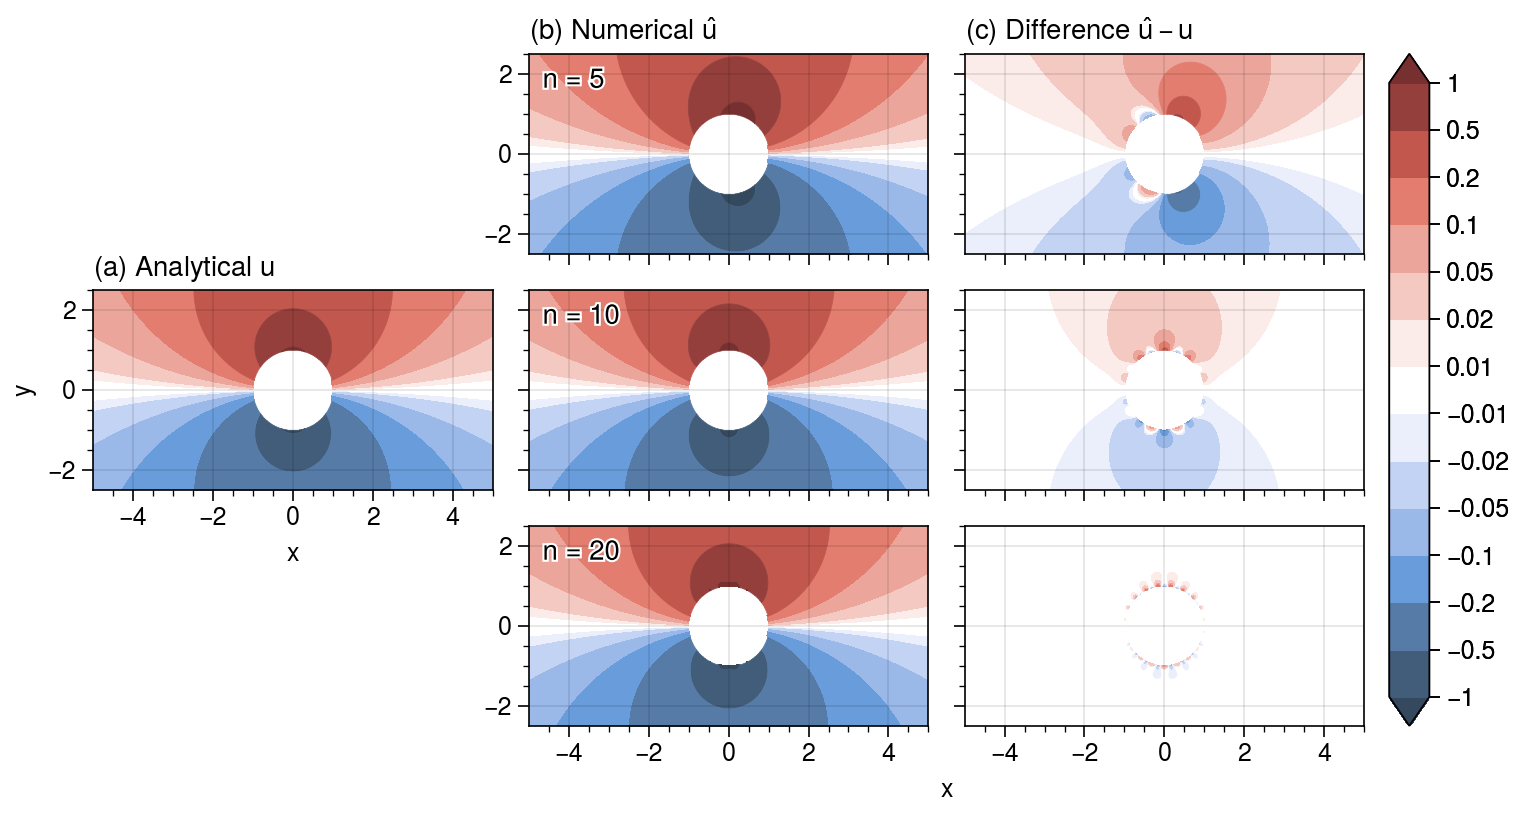
\includegraphics[width=\textwidth]{figures/prj3_qn1d_field.png}\\
    \caption{}
    \label{prj3_qn1d_field}
    \end{figure*}
    
    For test circles with radii (i) $1+\frac{1}{4}$, (ii) $1+\frac{1}{16}$ and (iii) $1+\frac{1}{256}$, we plot the errors for $n$ test points against $n$ in Fig. \ref{prj3_qn1dqn2b}a.  We see that the convergence rate for (i) and (ii) are largely of 2nd-order convergence.  However, (iii) order of convergence is non algebraic until around $n=1500$ where the order of convergence then transitions to 2nd order.

    \begin{figure*}[h!]
    \centering
    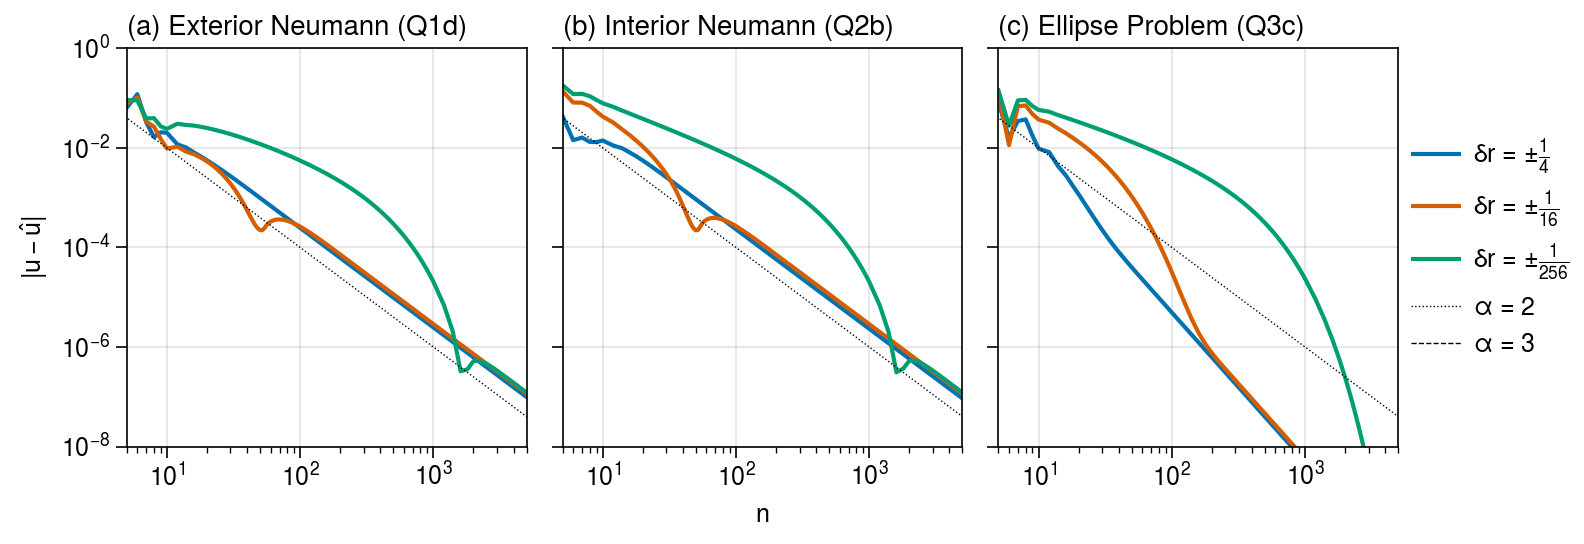
\includegraphics[width=0.8\textwidth]{figures/prj3_converge.png}\\
    \caption{}
    \label{prj3_converge}
    \end{figure*}
    
\end{enumerate}